\documentclass[11pt,preprint]{aastex}
%\documentstyle[11pt,psfig,aaspp4]{article}
\begin{document}

\def\simlt{\lower.5ex\hbox{$\; \buildrel < \over \sim \;$}}
\def\simgt{\lower.5ex\hbox{$\; \buildrel > \over \sim \;$}}

%{\noindent Astronomy 121 \hfill 2005jan18}

\title {UPDATE OF SECTION 6 OF THE LAB WRITEUP \\ \today}

The original version of section 6 was a bit muddled, so here's an
update. Use these two sections to replace the original section 6.


\section{MEASURING 1-D BRIGHTNESS DISTRIBUTIONS: THE FIRST STEP OF
MAKING MAPS} \label{mun}

	When we think of a time-variable signal, we think of frequency
as being cycles per second---and its inverse, the period, is in seconds,
the number of seconds that separates adjacent peaks of the sine wave. 

	The interferometer projects a giant sine wave on the sky. Its
frequency, which changes with position, is measured in cycles per
radian---and its inverse, the period, is the angular separation of
adjacent peaks, measured in the angular units of radians. You can, of
course, also think of frequency in terms of cycles per degree or cycles
per arcminute, with the corresponding periods (``fringe separation'') in
units of degrees or arcminutes. 

	When we observe with a range of baseline lengths and
orientations, the giant sine waves in the sky have corresponding ranges
of frequencies and orientations. We sample brightness of the sky in {\it
Fourier} space. The fringes at each baseline length and orientation have
amplitudes and phases. To recover the brightness of the sky in {\it
real, angular} space, we measure as many Fourier components as we can
and take their Fourier transform. If we had complete sampling in Fourier
space, we would recover the true brightness distribution. In real life,
we have {\it in}complete sampling, so we recover a distorted
representation of the true distribution. There is a whole literature 
of techniques for minimizing this distortion, the most prominent being
``cleaning'' and ``maximum entropy''. Full-fledged research arrays, such
as the Very Large Array (VLA) in New Mexico, rely on these techniques to
map the sky.

	In our case we have just two dishes along an east-west line. The
effective baseline length changes as the source rises higher in the sky,
and as long as the source is away from declination $\delta = 0^\circ$ the
orientation of the baseline also changes, at least to some degree. We
will map the Sun and Moon, which never get very far from $\delta =
0^\circ$, so effectively we have only a 1-d sampling of the source with
a range of baseline lengths. 

	Figure 1 illustrates this 1-d concept. It presents a generic
circular  source of uniform brightness in the sky, which we call the
MUN---a bastardization of the MOON and the SUN\footnote{In truth, it
represents neither, because neither the Sun nor the Moon have uniform
surface brightness.}. The top panel shows the MUN in the sky as it
really is: the fringes cover the 2-d object. At the bottom, we integrate
along vertical strips to get the 1-d brightness distribution---the
vertically-integrated 1-d equivalent, in which both the brightness
distribution and the fringes depend on only one coordinate. 

	This one coordinate is the horizontal direction in the bottom
panel of the Figure. In real life this is hour angle because we have an
east-west interferometer and our source is at low declination---meaning
that the baseline projected on the sky is mainly east-west, the
direction of hour angle. Thus we denote this direction by the letter
$h$. 

\begin{figure}[h!]
\begin{center}
\includegraphics[width=3.0in] {interf_fig.ps}
\end{center}
                                                                                
\caption{The 2-d and 1-d MUN. At the top, we see the situation in the
sky as it really is: the fringes cover the 2-d object.
At the bottom, we integrate along vertical strips to get the 1-d
brightness distribution and, also, the fringe amplitude (which goes from
--1 to +1). 
\label{interf_fig} } \end{figure}

	As the sky rotates, the source moves through the fringe pattern
to give the fringe response $R(t)$. The time $t$ is the same as the hour
angle $h$. For a point source, $R(h)= F(h)$; for an extended source, we
have to integrate over the extent of the source.  Let $I(h - h_s)$ be
the 1-d intensity distribution in the sky. That is, on the bottom panel
of Figure 1, $I(h - h_s)$ is the intensity of the source (vertical
direction) and $h-h_s$ the horizontal coordinate---the hour angle $h$
relative to the hour angle of the source center $h_s$. To be precise,
the source center is the intensity-weighted mean of the position, i.e.

\begin{equation}
h_s = { \int I(h)h dh \over \int I(h) dh} \ .
\end{equation}

	Now at any one time (hour angle $h$) the fringe pattern $F(h)$
covers the source and the interferometer response $R(h_s)$ is the integral
of the fringe pattern times the source intensity distribution, so we
have

\begin{equation}
R(h_s) = \int F(h) I(h-h_s) \ d h
\end{equation}

\noindent Now write $U = \left( {B_y \over \lambda} \cos\delta \right)$
and use equation \ref {fringeresponse} to write

\begin{equation} \label{r0}
R(h_s) = A \int I(h-h_s) \cos( 2\pi U \sin h) \ dh +  
	B \int I(h-h_s) \sin( 2\pi U \sin h) \ dh
\end{equation} 

	Our source occupies a small angle, so we can expand $h$ around $h_s$
by writing $[\Delta h = h-h_s]$. We use equation \ref{taylorexpansion} to
expand $\sin h$ as $\sin h \approx \sin( h_s) + \Delta h \cos( h_s)$.
Things are getting algebraically cumbersome, so let's eliminate
clutter by defining 

\begin{mathletters}
\begin{equation}
\alpha(h_s) = 2 \pi U \sin(h_s) 
\end{equation}
\begin{equation}
\beta(h_s, \Delta h) = 2 \pi U \cos(h_s) \  \Delta h = 2 \pi f_f \Delta h
\end{equation}
\end{mathletters}

\noindent [where $U = \left( {B \over \lambda} \cos\delta \right)$] so that equation \ref{r0} becomes

\begin{equation} \label{r1}
R(h_s) = A \int I(h-h_s) \cos( \alpha + \beta) \ dh +  
	B \int I(h-h_s) \sin( \alpha + \beta) \ dh
\end{equation} 

\noindent Now, as usual, we use trig identities [$\cos(\alpha + \beta) =
  \cos(\alpha) \cos(\beta) - \sin(\alpha) \sin(\beta)$ and $\sin(\alpha
  + \beta) = \sin(\alpha) \cos(\beta) + \cos(\alpha) \sin(\beta)$]. The
  first (cosine) term of equation \ref{r1} becomes

\begin{equation}
R^{\cos}(h_s) = A \; \cos(\alpha) \int I(\Delta h) \cos( \beta) \ d \Delta h 
-A \; \sin(\alpha) \int I(\Delta h) \sin( \beta) \ d \Delta h 
\end{equation}

\noindent with an equivalent, similar expression for $R^{\sin}(h_s)$. We
imagine $I(\Delta h)$ as being composed of little slices in hour angle,
with each little slice of the source characterized by its position
offset $\Delta h$ and its intensity $I(\Delta h)$. For our source (the
MUN), we assume the that $I(\Delta h)$ is symmetric (This also retains
our algebraic sanity). This means that in the above equation the second
term, which is antisymmetric, integrates to zero.  Similarly, the
antisymmetric term in the equivalent equation $R^{\sin}(h_s)$ also
integrates to zero, so we end up with $R(h_s) = R^{\cos}(h_s) +
R^{\sin}(h_s)$, or

\begin{equation} \label{interfeqn}
R(h_s) = 
\underbrace{ \left\{ A \; \cos[\alpha(h_s)]
\ + B \; \sin[\alpha(h_s)]
\right\}}_{Point-source\ 
Fringe} \times 
\underbrace{\int I(\Delta h) \cos[ \beta(h_s,\Delta h)] \ d \Delta h}_{Fringe \ Modulator} 
\end{equation}


	Note the structure of equation \ref{interfeqn}. It consists of
two factors. The first ``Point-source Fringe'' term is identical to equation
\ref{fringeresponse}---it's the response to a point source located at
$\Delta h=0$. The other modulates (multiplies) this function. 

Generally, {\it the modulating function is the Fourier transform of the
  source intensity distribution on the sky}. 
Here, we assumed a
one-dimensional source; more generally, the Fringe Modulator depends on
the two-dimensional map of intensity on the sky, so it's a double
integral instead of a single one. We also assumed a symmetric source,
  which means that the sine portion of the Fourier
  transform is zero; this is why equation \ref{interfeqn} is only a cosine
  Fourier transform instead of a full one.

\begin{figure}[h!]
\begin{center}
\includegraphics[width=3.5in] {cosfringe.ps}
\end{center}
                                                                                
\caption{Examples of 1-d brightness distributions and their Fourier
transforms. Top panel: the brightness distributions. Bottom: the Fourier
transforms. In both, panels, the solid line is for a flat brightness
distribution and the dashed one for a cosine distribution. 
\label{cosfringe} } \end{figure}

Figure \ref{cosfringe} (top panel) shows two examples of 1-d brightness
distributions, a flat and a cosine distribution.  The bottom panel shows
the Fourier transforms.  Both of the modulating functions are trig
functions. In particular, for the flat distribution the modulating
function is ${ \sin(2 \pi f_f R) \over 2 \pi f_f R}$. It can (and does!)
go through zero. {\it The locations of these zero points provide crucial
information about the source structure}. The zeros occur for $f_f={n
\over 2R}$. It's more intuitive to express the zeros in terms of fringe
{\it period} (equal to $1 \over f_f$): the zeros occur at $Period = {2R
\over n}$. There's a zero whenever there's an integral number of fringe
periods over the source width. This makes perfect sense, because then
the source contributes equally to the negative and positive portions of
the fringe and the net integral is zero.

\section{MEASURING THE DIAMETER OF A CIRCULAR SOURCE}

Our goal is to measure and compare the diameters of the Sun and
Moon. We'll make the assumption that the sources are uniformly-bright
disks of radius $R$, which means

\begin{equation}
I(\Delta h) = { (R^2 - \Delta h^2)^{1/2} \over  R}
\end{equation}

\noindent To obtain the theoretical modulating function $MF_{theory}$, you use the integral in
equation \ref{interfeqn}, which is

\begin{equation}
MF_{theory} = {1 \over R} \int_{-R}^R (R^2 - \Delta h^2)^{1/2} 
	cos(2\pi f_f \Delta h) d \Delta h
\end{equation}

\noindent If you want, you can do this analytically by substituting $R
\cos (\theta)$ for $\Delta h$; you end up with a Bessel function. We are
running a lab class, not a math class, so let's proceed by doing the
integral {\it numerically}! To accomplish this, split $I(\Delta h)$ into
$2N + 1$ tiny little slices (the total number is odd, which makes the
slices symmetric about $\Delta h = 0$). Each slice has width $\delta h =
{R \over N}$, and $\Delta h_n = n \delta h$, where $n$ runs from $-N$ to
$+N$. Then the integral becomes a sum:

\begin{equation}
MF_{theory} \approx {1 \over R} \sum_{n=-N}^{n=+N}
[R^2 - (n \delta h)^2]^{1/2} \cos(2 \pi f_f n\delta h) \delta h
\end{equation}

\noindent which we rewrite as

\begin{equation}
MF_{theory} \approx  \delta h \sum_{n=-N}^{n=+N}
\left[ 1 - \left( n \over N\right)^2 \right]^{1/2} 
\cos \left( 2 \pi f_f R n \over N \right)
\end{equation}

\noindent Note the important point that $MF_{theory}$ is a function {\it only} of
the combination $f_f R$. Thus, for this model you can theoretically
determine the particular values of $f_f $ for which $MF_{theory} = 0$. Your
observations give you the value of $f_f$ (or, equivalently, the hour
angle) for which the observed $MF_{obs}$ is zero. Combining these gives
you the source size. 


\end{document}

